\documentclass[11pt,a4paper]{article}

% Compile with pdfLaTeX (the Overleaf default). Upload the figures/ folder too.
\usepackage[utf8]{inputenc}
\usepackage[T1]{fontenc}
\usepackage[english]{babel}
\usepackage{lmodern}
\usepackage{microtype}
\usepackage[a4paper,margin=2.3cm]{geometry}
\usepackage{amsmath}
\usepackage{graphicx}
\usepackage{booktabs}
\usepackage{tabularx}
\usepackage{array}
\usepackage{float}
\usepackage{caption}
\usepackage{xcolor}
\usepackage{listings}
\usepackage{tikz}
\usetikzlibrary{arrows.meta,positioning,fit}
\usepackage[hidelinks]{hyperref}

\graphicspath{{figures/}}
\captionsetup{font=small,labelfont=bf}
\setlength{\parskip}{5pt}
\setlength{\parindent}{0pt}
\setlength{\emergencystretch}{3em}
% A page of floats starts at the top, not in the middle.
\makeatletter\setlength{\@fptop}{0pt}\makeatother
\renewcommand{\arraystretch}{1.15}

\definecolor{wrong}{HTML}{B42828}
\definecolor{notebg}{HTML}{F3F2EE}
\definecolor{blue}{HTML}{2A78D6}
\definecolor{orange}{HTML}{EB6834}
% Red marker for every value that still has to be filled in from your own results.
% Search the file for TODO before handing the report in.
\newcommand{\TODO}[1]{\textcolor{wrong}{\textbf{[TODO: #1]}}}
\newcommand{\fig}[2]{\IfFileExists{figures/#1}{\includegraphics[width=#2]{#1}}%
  {\fbox{\parbox{0.9\linewidth}{\centering\vspace{2em}\TODO{figure \detokenize{#1} not generated yet}\vspace{2em}}}}}
\newcommand{\notebox}[1]{\par\smallskip\noindent\colorbox{notebg}{\parbox{\dimexpr\linewidth-2\fboxsep}{\small #1}}\par\smallskip}
\newcommand{\code}[1]{{\frenchspacing\texttt{#1}}}

\lstset{basicstyle=\ttfamily\footnotesize,columns=fullflexible,keepspaces=true,
        frame=single,rulecolor=\color{black!25},backgroundcolor=\color{notebg},
        xleftmargin=3pt,xrightmargin=3pt,breaklines=true}
\lstdefinelanguage{CSharp}{morekeywords={public,private,sealed,class,record,static,readonly,var,new,return,
  lock,try,catch,throw,await,async,foreach,if,else,while,using,string,long,bool,void,null,true,false,in,is,not,
  override,yield,internal},sensitive=true,morecomment=[l]{//},morestring=[b]"}
\lstdefinelanguage{Proto}{morekeywords={syntax,package,import,service,rpc,returns,stream,message,optional,repeated,
  int64,int32,string,option},sensitive=true,morecomment=[l]{//},morestring=[b]"}

\begin{document}

% Title
\begin{center}
  {\small NETWORK PROGRAMMING \textperiodcentered{} UTM}\\[6pt]
  {\LARGE\bfseries Laboratory Work 4: A Message Broker}\\[10pt]
  \begin{tabular}{rl}
    Authors: & Pancenco Ina, Rusnac Nichita \\
    Group:   & FAF-242 \\
    Teacher: & Ernest B\^{\i}tca \\
    Date:    & November 2026
  \end{tabular}
\end{center}
\vspace{4pt}\hrule\vspace{8pt}

% Section 1
\section{The task and the environment}

A message broker is the program in the middle of many distributed systems. Publishers send messages
to a \emph{topic} (a named channel such as \code{grades} or \code{news}); the broker gives each
message an id (1, 2, 3, \dots{} in each topic) and the time, keeps it, puts it in a queue and
delivers it in the background to every subscriber of that topic. Publishers and subscribers know
only the address of the broker, never each other, so either side can stop, change or multiply
without the other noticing.

The laboratory work has two parts with the same three tasks each: \emph{publish and deliver},
\emph{restarts} (nothing is lost when the broker restarts) and \emph{strangers} (only publishers with
a token may publish). In Part~1 the broker speaks HTTP: a REST API with JSON, built on
\code{HttpListener} of the .NET standard library, and a subscriber receives the messages over an
answer that stays open. In Part~2 it speaks gRPC: the same broker, with the contract written in
Protocol Buffers and a server stream for each subscriber.

Everything is written in C\# for .NET~9. Part~1 is a command of the same \code{Labs} program as the
previous laboratory works (\code{Labs.exe lab4 broker}); Part~2 is a project of its own,
\code{lab4/grpc/BrokerGrpc.csproj}, because its broker runs on Kestrel (ASP.NET Core), which Part~1
must not use. The part of the broker that does not depend on the network (the store, the queue,
the delivery, the tokens and the log) is in the folder \code{lab4/Core} and is compiled into both
projects, so Part~2 really is ``the same broker'': only the way the programs talk changes. No
existing broker and no messaging library is used; the only packages are \code{Grpc.AspNetCore} and
\code{Grpc.Net.Client} in Part~2.

The tests ran on one Windows~11 computer with .NET SDK 9.0.321 and Python 3.13; the measurements are
from the same computer, with the broker and the clients on the loopback interface.

% Section 2
\section{Design}

\subsection{Programs}

There are three console programs, as the task asks: the \emph{broker}, the \emph{publisher} and the
\emph{subscriber}. As in the previous labs they are commands of one executable, but each runs as its
own process, any number of them, on any computer:

\begin{lstlisting}
Labs.exe lab4 broker    --port 8080 [--data <folder>] [--tokens <file>] [--log <file>]
Labs.exe lab4 publish   --broker http://192.168.1.5:8080 --topic grades --name teacher [--token <token>]
Labs.exe lab4 subscribe --broker http://192.168.1.5:8080 --topic grades [--after <id>] [--ids]
Labs.exe lab4 topics    --broker http://192.168.1.5:8080
Labs.exe lab4 bench     --broker http://192.168.1.5:8080 --messages 1000 --publishers 8
BrokerGrpc.exe broker | publish | subscribe | topics | bench     (Part 2, the same options, port 50051)
\end{lstlisting}

The publisher publishes every line the user types and prints the id that the broker gave it. The
subscriber shows each message as it arrives, in order, in the format of the task:

\begin{lstlisting}
[grades] teacher: Lab 3 grades are online
\end{lstlisting}

\code{topics} prints the list of topics, and \code{bench} runs several publishers at the same time
against one topic while a subscriber listens, and checks the ids and the delivery
(Section~\ref{sec:measure}).

The client programs are written once, in \code{Core/ClientPrograms.cs}, against a small interface
\code{IBrokerClient} with three methods: publish, subscribe, list the topics. Part~1 implements it
with \code{HttpClient} (\code{HttpBrokerClient}), Part~2 with the client class generated from the
\code{.proto} file (\code{GrpcBrokerClient}).

\subsection{The broker: producers, a queue, a consumer}

Figure~\ref{fig:arch} shows the inside of the broker. Every request is handled on a task of its own,
so many clients are served at the same time. A publish is a \emph{producer}: it gives the message
its id and time, saves it, puts it in the queue and answers at once. The \emph{delivery task} is the
single \emph{consumer}: it takes the messages out of the queue in order and offers each one to every
subscriber of its topic, as in the producer--consumer pattern of Lecture~3. The queue is a
\code{Channel<BrokerMessage>} from \code{System.Threading.Channels}, a thread-safe queue whose reader
can wait for the next item without blocking a thread.

\begin{figure}[H]
\centering
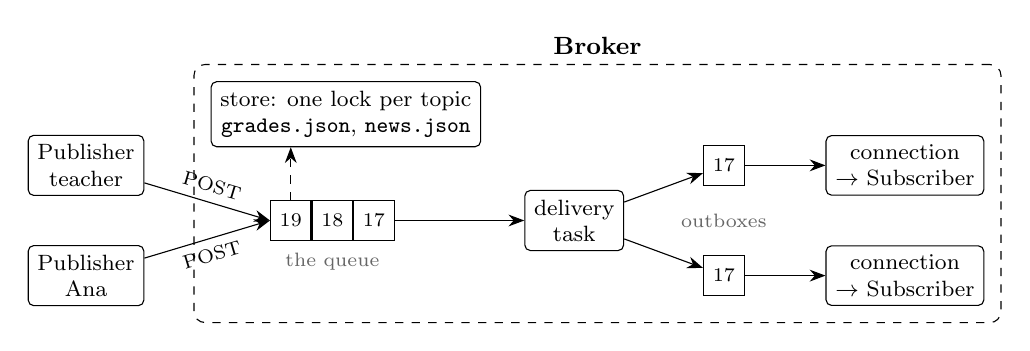
\begin{tikzpicture}[font=\footnotesize, >={Stealth[length=2mm]},
  box/.style={draw, rounded corners=2pt, minimum height=7mm, align=center, fill=white},
  q/.style={draw, minimum width=5mm, minimum height=5mm, font=\scriptsize}]
  \node[box] (p1) at (0,0.7) {Publisher\\teacher};
  \node[box] (p2) at (0,-0.7) {Publisher\\Ana};
  \node[box] (store) at (3.3,1.35) {store: one lock per topic\\\code{grades.json}, \code{news.json}};
  \node[q] (q3) at (2.6,0) {19};
  \node[q, right=0pt of q3] (q2) {18};
  \node[q, right=0pt of q2] (q1) {17};
  \node[font=\scriptsize, below=1pt of q2, text=black!60] {the queue};
  \node[box] (d) at (6.2,0) {delivery\\task};
  \node[q] (o1) at (8.1,0.7) {17};
  \node[q] (o2) at (8.1,-0.7) {17};
  \node[font=\scriptsize, text=black!60] at (8.1,0) {outboxes};
  \node[box] (s1) at (10.4,0.7) {connection\\$\to$ Subscriber};
  \node[box] (s2) at (10.4,-0.7) {connection\\$\to$ Subscriber};
  \node[draw, rounded corners=4pt, dashed, inner sep=6pt, fit=(store)(q3)(q1)(d)(o1)(o2)(s1)(s2), label={[font=\small\bfseries]above:Broker}] {};
  \draw[->] (p1) -- node[above, sloped, font=\scriptsize] {POST} (q3.west);
  \draw[->] (p2) -- node[below, sloped, font=\scriptsize] {POST} (q3.west);
  \draw[->, dashed] (q3.north) ++(0,0) -- (store.south west -| q3.north);
  \draw[->] (q1) -- (d);
  \draw[->] (d) -- (o1);
  \draw[->] (d) -- (o2);
  \draw[->] (o1) -- (s1);
  \draw[->] (o2) -- (s2);
\end{tikzpicture}
\caption{A publish saves the message and puts it in the queue (producer). The delivery task takes it out
(consumer) and puts it in the outbox of every subscriber of its topic; the connection of each subscriber
writes its outbox to the network.}\label{fig:arch}
\end{figure}

\subsection{Ids, order and the lock of a topic}

Two publishers that publish to the same topic at the same time must never get the same id and never
lose a message. Each topic in \code{MessageStore} has its own lock; the id, the save to disk and the
write into the queue all happen while that lock is held:

\begin{lstlisting}[language=CSharp]
lock (topic.Lock)
{
    var message = new BrokerMessage(topic.LastId + 1, topicName, sender, body, DateTimeOffset.UtcNow);
    topic.Messages.Add(message);
    // Task 2: on the disk before the answer; if it cannot be saved, it is taken back and its id is not used
    try { Save(topicName, topic.Messages); }
    catch { topic.Messages.RemoveAt(topic.Messages.Count - 1); throw; }
    topic.LastId = message.Id;
    accepted(message);   // into the queue, still in the lock
    return message;
}
\end{lstlisting}

Because the queue receives the messages of a topic while the lock is held, it receives them in the
order of their ids, and the single delivery task keeps that order. Publishes to \emph{different}
topics do not wait for each other. A message that cannot be saved is taken back, so the ids have no
gaps, and the publisher gets an error instead of a \code{202}.

\subsection{Subscribers, outboxes, and subscribers that are gone}

A subscriber is a \code{Subscription} with an \emph{outbox}: a bounded channel of 1\,000 messages.
The delivery task only puts messages into outboxes, which never waits; the connection of each
subscriber (an HTTP answer in Part~1, a gRPC stream in Part~2) takes them out and writes them to the
network. So a slow subscriber cannot hold up the delivery to the others. Two kinds of subscribers
are forgotten:

\begin{itemize}
\item \textbf{Gone}: its connection is closed or broken, so a write fails. The connection logs the
  failure, unregisters the subscriber and ends. A dead connection that receives nothing is found by
  the heartbeat (Part~1) or the HTTP/2 keep-alive pings (Part~2), every 15\,s.
\item \textbf{Too slow}: its outbox is full (it is 1\,000 messages behind). The delivery task drops it
  and aborts its connection, so a write that hangs is stopped as well.
\end{itemize}

When a subscriber connects it can ask for the stored messages after an id (\code{?after=17} in
Part~1, \code{after\_id} in Part~2): this is how a subscriber comes back after a restart without
missing messages. The broker first registers the subscriber, and only then reads the stored messages
after that id. A message published in between is in both places, and the subscription sends each id
only once (it remembers the last id it sent); no message can fall between the two.

\subsection{The log}

The broker writes a line for every request and every delivery, on the console and in
\code{lab4/logs/broker-http.log} (or \code{broker-grpc.log}): the time, the client (its endpoint),
the request, the topic, the id of the message and the result. A lock keeps the lines of different
threads apart. A part of the log of a test, with a subscriber that left without a word:

\begin{lstlisting}
15:57:22.289  [::1]:63906   GET /topics/news/stream     topic=news  id=-  200 OK, subscribed
15:57:22.637  [::1]:63907   GET /topics/news/stream     topic=news  id=-  200 OK, subscribed
15:57:23.259  [::1]:63909   POST /topics/news/messages  topic=news  id=1  202 Accepted, from ana
15:57:23.267  [::1]:63906   DELIVER                     topic=news  id=1  delivered
15:57:23.268  [::1]:63907   DELIVER                     topic=news  id=1  failed, the subscriber is gone
                                                                          and forgotten (...)
15:57:23.272  [::1]:63910   POST /topics/news/messages  topic=news  id=2  202 Accepted, from ana
15:57:23.273  [::1]:63906   DELIVER                     topic=news  id=2  delivered
\end{lstlisting}

% Section 3
\section{Part 1: the broker over HTTP}

\subsection{Task 1: Publish and deliver}

The broker is an \code{HttpListener}; there is no web framework. A loop accepts the requests and
starts a task for each one; the path is split into its segments and matched against the three
routes of the API (Table~\ref{tab:api}). Every body is JSON; the publisher sends \code{sender} and
\code{body}, and the broker adds \code{id}, \code{topic} and \code{time} to every message it answers
with or forwards:

\begin{lstlisting}
POST /topics/grades/messages
{"sender":"teacher","body":"Lab 3 grades are online"}

202 Accepted
{"id":17,"topic":"grades","sender":"teacher","body":"Lab 3 grades are online","time":"2026-11-23T13:53:03.2000167+00:00"}
\end{lstlisting}

\begin{table}[H]
\centering\small
\caption{The HTTP API of the broker.}\label{tab:api}
\begin{tabularx}{\linewidth}{@{}llXl@{}}
\toprule
Request & & What it does & Answer \\
\midrule
\code{POST} & \code{/topics/\{topic\}/messages} & queues a message & \code{202 Accepted} + the message \\
\code{GET} & \code{/topics/\{topic\}/stream} & new messages, as they arrive (\code{?after=id}: first the stored ones after id) & \code{200 OK}, stays open \\
\code{GET} & \code{/topics} & the topics, with their sizes, last ids and subscribers & \code{200 OK} \\
\bottomrule
\end{tabularx}
\end{table}

\textbf{The stream.} A subscription is an answer that is never finished. It is sent with
\code{Transfer-Encoding: chunked} (\code{SendChunked = true}), so it needs no length, and every
message is one line of JSON (NDJSON, \code{application/x-ndjson}). Each line is written and flushed
as soon as the message comes out of the outbox. After 15\,s without messages the broker writes an
empty line, a \emph{heartbeat}: if the subscriber is gone, that write fails and the subscriber is
forgotten; if the broker is gone, the subscriber notices that nothing came for 45\,s. The header
\code{Last-Id} tells the subscriber after which id its messages start. The client reads the stream
with \code{HttpCompletionOption.ResponseHeadersRead}, which gives the answer as soon as its headers
arrive, and then reads it line by line.

\textbf{Errors.} A request that the broker cannot accept gets a status code and a JSON body
\code{\{"error": "..."\}}, and a line in the log. Every request runs inside a \code{try}; an
unexpected exception becomes a \code{500}, so the broker never crashes because of a request.

\begin{table}[H]
\centering\small
\caption{The errors of Part 1, and of Part 2 for the same cases.}\label{tab:errors}
\begin{tabularx}{\linewidth}{@{}Xll@{}}
\toprule
Case & HTTP (Part 1) & gRPC (Part 2) \\
\midrule
topic name not valid, body not JSON or not an object, \code{sender} or \code{body} missing or too long, \code{after} negative & \code{400 Bad Request} & \code{InvalidArgument} \\
no token, unknown token, or another scheme than \code{Bearer} (Task 3) & \code{401} + \code{WWW-Authenticate: Bearer} & \code{Unauthenticated} \\
good token, topic not allowed (Task 3) & \code{403 Forbidden} & \code{PermissionDenied} \\
unknown path & \code{404 Not Found} & \code{Unimplemented} (by gRPC) \\
known path, wrong method & \code{405} + \code{Allow} & --- \\
body larger than 64\,KB & \code{413 Content Too Large} & \code{ResourceExhausted} (by gRPC) \\
the message could not be saved & \code{503 Service Unavailable} & \code{Unavailable} \\
any other exception & \code{500 Internal Server Error} & \code{Internal} \\
\bottomrule
\end{tabularx}
\end{table}

\subsection{Task 2: Restarts}

Every topic is one file, \code{lab4/data/http/<topic>.json}, with all its messages. A publish
writes the whole topic to \code{<topic>.json.tmp}, forces it to the disk (\code{Flush(true)}), and
then renames it over \code{<topic>.json} (\code{File.Move(..., overwrite: true)}). Only after that
does the broker answer \code{202}. A rename inside one folder replaces the old file in one step, so a
broker killed at any moment leaves either the old file or the new one, never a half-written one. A
leftover \code{.tmp} is the trace of a write that did not finish; the next start deletes it. At the
start the broker reads every topic file, and the ids go on from the last one.

The clients survive a restart too. A publisher whose message cannot reach the broker
(\code{HttpRequestError.ConnectionError}: the connection could not even be made, so the request was
never sent and sending it again cannot create a duplicate) tries again every second for up to 30\,s.
A subscriber whose stream ends connects again, with \code{?after=} the last id it has shown, so it
gets the messages it missed while the broker was down, and none twice. A restart, as the subscriber
and the publisher showed it (long lines cut):

\begin{lstlisting}
[grades] teacher: before the restart
(connection lost: Unable to read data from the transport connection: An existing connection was
 forcibly closed by the remote host; trying again in 1 s)
(cannot connect: No connection could be made because the target machine actively refused it.
 (localhost:18150); trying again in 2 s)
(connected again to http://localhost:18150)
[grades] teacher: while the broker is down
\end{lstlisting}
\begin{lstlisting}
  -> #1 at 18:14:43.774
  the broker is not reachable (No connection could be made because the target machine actively
  refused it. (localhost:18150)), trying again every second...
  -> #2 at 18:14:51.099
\end{lstlisting}

\notebox{Rewriting the whole topic for every message keeps the format simple (one JSON array per
topic, easy to read at the defense) and the replace safe, but it costs time proportional to the size
of the topic. A real broker appends to a log file and replaces only small index files; for the
sizes of this lab the simple way is enough, and Section~\ref{sec:measure} shows what it costs.}

\subsection{Task 3: Strangers}

With \code{-{}-tokens lab4/tokens.json} only known publishers may publish. The file lists the
publishers, each with its token and the topics it may publish to (\code{"*"} for all):

\begin{lstlisting}
{ "publishers": [
    { "name": "teacher", "token": "teacher-5f2c9a71d3", "topics": ["grades", "news"] },
    { "name": "Ana",     "token": "ana-8b41e07c66",     "topics": ["news"] } ] }
\end{lstlisting}

The token comes in the header \code{Authorization: Bearer <token>}. Without a token, with another
scheme or with an unknown token the publish gets \code{401 Unauthorized} with
\code{WWW-Authenticate: Bearer}; with a known token but a topic it does not allow, \code{403
Forbidden}. The difference matters: 401 means ``I do not know who you are'', 403 ``I know you, and
you may not''. With tokens, the sender of a message is the name of the token's publisher, whatever
the body says, so nobody can publish under somebody else's name. The broker reads the file again
when its modification time changes, so publishers can be added or removed while it runs; a file
that cannot be read (half saved by an editor) is ignored and the old tokens are kept. Subscribing
and listing the topics need no token: the task protects publishing.

% Section 4
\section{Part 2: the broker over gRPC}

\subsection{The contract}

In Part~1 every program had to agree by hand on the methods, the paths, the status codes and the
fields of the JSON. In gRPC this agreement is a contract, \code{lab4/grpc/broker.proto}; the classes
of the messages, the base class of the server and the client are generated from it at build time by
\code{Grpc.Tools}. The service starts as the task gives it; the other messages are ours:

\begin{lstlisting}[language=Proto]
service Broker {
  rpc Publish (PublishRequest) returns (PublishReply);           // one request, one answer
  rpc Subscribe (SubscribeRequest) returns (stream Message);     // a stream of answers
  rpc ListTopics (ListTopicsRequest) returns (ListTopicsReply);  // the topics, and their sizes
}
message PublishRequest   { string topic = 1; string sender = 2; string body = 3; }
message PublishReply     { int64 id = 1; google.protobuf.Timestamp time = 2; }
message SubscribeRequest { string topic = 1; optional int64 after_id = 2; }
message TopicInfo        { string name = 1; int64 size = 2; int64 last_id = 3;
                           int32 subscribers = 4; }
message ListTopicsReply  { repeated TopicInfo topics = 1; }
\end{lstlisting}

\code{after\_id} is \code{optional}, so ``not set'' (only new messages) is different from 0 (every
stored message). The numbers after the fields are their tags on the wire: a field can be added later
with a new tag, and old programs simply ignore it.

\subsection{Task 1: Publish and deliver}

\code{BrokerService} overrides the three calls of the generated \code{Broker.BrokerBase} and uses the
same \code{MessageBroker} as Part~1. \code{Publish} is unary: it checks the request, saves and queues
the message and answers at once with its id and time. \code{Subscribe} is server streaming: it
registers the subscriber, sends the response headers at once (with \code{last-id}, as in Part~1), and
then writes every message of the outbox into the stream with \code{IServerStreamWriter.WriteAsync},
for as long as the stream is open. When the subscriber goes away, gRPC cancels the call
(\code{context.CancellationToken}) and the subscriber is forgotten. There is no heartbeat of our
own: Kestrel sends HTTP/2 keep-alive pings every 15\,s on an idle connection, and the client does
the same, so a dead connection is found from both sides. \code{ListTopics} answers with the topics.

The broker listens on HTTP/2 only, without TLS, and maps only the gRPC service: in this part it has
no HTTP API (a test checks that \code{GET /topics} gets no answer of the API). All the calls of
one client share one HTTP/2 connection, each as a stream of its own.

\subsection{Tasks 2 and 3}

Task~2 needs no new code: the store, the files and the clients that come back are the same as in
Part~1 (the gRPC subscriber connects again with \code{after\_id}; a publish that fails with
\code{Unavailable} is tried again). Task~3 reads the token from the metadata
\code{authorization: Bearer <token>}, the gRPC form of the headers, with the same \code{TokenFile},
and answers \code{Unauthenticated} or \code{PermissionDenied} (Table~\ref{tab:errors}).

\subsection{HTTP and gRPC compared}

\begin{center}
\small
\begin{tabularx}{\linewidth}{@{}lXX@{}}
\toprule
 & Part 1: HTTP + JSON & Part 2: gRPC + Protobuf \\
\midrule
agreement & by hand: paths, methods, codes, JSON fields (in the README) & the \code{.proto} file; code generated from it \\
a publish & \code{POST}, answer \code{202} with the message & a method call, \code{PublishAsync(...)} \\
a subscription & a chunked answer that stays open, one JSON per line & a server stream of \code{Message} \\
dead connection & our heartbeat (an empty line every 15\,s) & HTTP/2 keep-alive pings \\
errors & status code + JSON \code{error} & status code + detail \\
token & header \code{Authorization} & metadata \code{authorization} \\
transport & HTTP/1.1, text & HTTP/2, binary, many calls on one connection \\
the message of Section 3.1 & 121 bytes of JSON (names and the time as text) & 57 bytes of Protobuf (tags and varints) \\
\bottomrule
\end{tabularx}
\end{center}

% Section 5
\section{Tests}\label{sec:tests}

The tests (\code{lab4/tests/test\_broker.py}) start real brokers, each with its own port, data folder
and log, and real publishers and subscribers, typed into through their standard input. For Part~1
they also send raw HTTP requests from Python, to send what the programs never send. Part~2 has no
HTTP API, so its tests use only the gRPC programs. All 14 tests passed (Table~\ref{tab:tests}).

\begin{table}[tbp]
\centering\small
\caption{The automatic tests.}\label{tab:tests}
\begin{tabularx}{\linewidth}{@{}lXc@{}}
\toprule
Test & What it checks & Result \\
\midrule
http publish and deliver & two publishers, two subscribers: ids 1, 2; both show both messages, in the format of the task; a subscriber of another topic gets nothing; \code{GET /topics} & passed \\
http api & \code{202} with the message; 10 bad requests (not JSON, an array, missing fields, bad topic, 70\,KB body, wrong methods, unknown path, negative \code{after}) answered 400, 413, 405 with \code{Allow}, 404, each with a JSON error and a log line; the broker goes on & passed \\
http concurrent publishers & 8 publishers, 600 messages at the same time: ids 1 to 600, each once; the subscriber gets all, once, in order & passed \\
http gone subscriber & a subscriber that closes its connection and one that is killed: the others get every message; the broker forgets both & passed \\
http restart & broker killed; the subscriber and the publisher come back by themselves; the message typed while the broker was down gets id 4; no message lost or shown twice; \code{?after=2} gives 3, 4, 5 & passed \\
http half-written file & a cut \code{.json.tmp} next to the topic file: deleted at the start, the ids go on & passed \\
http many restarts & the broker killed 5 times while a publisher sends without a pause: every acknowledged message is still there, the ids have no gaps & passed \\
http tokens & no token, unknown token, \code{Basic}: 401 + \code{WWW-Authenticate: Bearer}; topic not allowed: 403; the sender is the token's name; a token added to the file while the broker runs works & passed \\
grpc publish and deliver & the same as for HTTP, and \code{topics}; a bad topic name refused & passed \\
grpc concurrent publishers & 8 publishers, 600 messages: the same checks & passed \\
grpc gone subscriber & a killed subscriber: the other gets every message; the broker forgets it & passed \\
grpc restart & the same as for HTTP; \code{-{}-after 2} gives 3, 4, 5 & passed \\
grpc tokens & \code{Unauthenticated} without a token and with an unknown one, \code{PermissionDenied} for a topic not allowed, logged & passed \\
grpc has no HTTP API & \code{GET /topics} on the gRPC port gets no answer of the API & passed \\
\bottomrule
\end{tabularx}
\end{table}

In the test with five restarts in a row the publisher got a \code{202} for 193 messages, and all 193 were
in the topic after the last restart, with ids 1 to 193. The drop of a subscriber whose outbox is full
was not tested automatically: it needs a subscriber that stops reading while more than 1\,000
messages, plus the buffers of TCP, pile up.

\subsection{On two computers}\label{sec:two}

\TODO{At the defense: the broker on one computer, two publishers and two subscribers of one topic
spread over both computers (for Part~1 after the \code{netsh http add urlacl} and firewall commands of
the README). Write here the addresses, what the subscribers showed when both publishers typed at the
same time, and a few lines of the log with the endpoints of the other computer.}

% Section 6
\section{Measurements}\label{sec:measure}

\code{bench} subscribes to a topic and then publishes 1\,000 messages to it from 1 to 16 publishers
at the same time, each publisher sending its next message as soon as the previous one is answered.
It measures the time from a publish to its answer, the time from a publish to the arrival of the
message at the subscriber, and the throughput; and it checks that the ids are unique and without
gaps and that the subscriber got every message once, in order. Every case ran three times on a new
broker (Figure~\ref{fig:bench}); the checks passed in all 30 runs: 30\,000 messages, every id given
once and with no gaps, every message received once and in order.

\begin{figure}[H]
\centering
\fig{throughput.png}{0.49\linewidth}\hfill\fig{latency.png}{0.49\linewidth}
\caption{Left: messages published per second to one topic. Right: from a publish to its answer, median
(solid) and 99th percentile (dashed). The points are medians of three runs, the bars the lowest and the
highest run.}\label{fig:bench}
\end{figure}

\textbf{The throughput does not grow with the publishers}: about 177 messages per second with one
publisher, and 195 to 226 with 2 to 16, for both parts. The reason is the lock of the topic: a
publish holds it while it writes the whole topic to the disk and forces it there (\code{fsync}).
Measured alone, that save costs 2 to 3\,ms on this computer, and almost the same for half a kilobyte
as for 150\,KB, because the time goes into \code{fsync}, not into writing the bytes. So about 4.5\,ms
of every publish (save, serialisation, queue) happen one at a time, and one topic cannot take more
than about $1/4.5\,\text{ms} \approx 220$ messages per second, however many publishers wait. With one
publisher the throughput is a little lower, because nothing else is done while its request and answer
travel.

\textbf{The latency grows with the publishers} for the same reason: with $n$ publishers, a publish
waits for the $n-1$ in front of it, so the median is about $n \times 4.5$\,ms (35\,ms with 8, 65 to
78\,ms with 16). The 99th percentile is two to four times higher: \code{lock} in .NET is not a fair
queue, so an unlucky publisher can be passed several times, and \code{fsync} itself sometimes takes
longer.

\textbf{HTTP and gRPC are close.} With one publisher the latency is the same (4.9 and 5.1\,ms); with
more, HTTP published 3 to 15\% more messages per second, close to the spread between runs.
The transport is not the bottleneck here; keeping every message safe on the disk is. gRPC's smaller
messages (57 instead of 121 bytes) matter little on the loopback interface.

\textbf{Delivery is not a bottleneck}: the subscriber received each message 0.05 to 0.2\,ms
\emph{before} the publisher received its answer, because the message is in the queue, and the
delivery task gives it to the outbox, while the answer of the publisher is still being written.

The design chose safety over speed: a \code{202} means the message is on the disk. Without
\code{fsync}, or with one append-only file per topic and one \code{fsync} for several messages at
once (as real brokers do), the throughput would be many times higher, at the cost of more code or of
losing the last messages when the power fails. Different topics have different locks, so they are
saved in parallel; the benches used one topic, the worst case.

% Section 7
\section{Where to change what}\label{sec:change}

At the defense the teacher may ask for a small change. The places:

\begin{center}
\small
\begin{tabularx}{\linewidth}{@{}>{\raggedright\arraybackslash}p{0.3\linewidth}>{\raggedright\arraybackslash}X@{}}
\toprule
Change & Where \\
\midrule
a new field in the messages (for example \code{priority}) &
  \code{Core/BrokerMessage.cs}: add it to \code{BrokerMessage} and \code{PublishBody};
  \code{Core/MessageStore.cs} (\code{Add}) and \code{MessageBroker.Publish}: pass it on;
  Part~1: \code{HttpBroker.PublishAsync} passes \code{body.Priority} (the JSON follows by itself);
  Part~2: \code{broker.proto} (a new tag in \code{PublishRequest} and \code{Message}),
  \code{BrokerService.Publish} and \code{ToProto}, \code{GrpcBrokerClient}; and \code{ClientPrograms.Format} to show it \\
another time limit & \code{Core/BrokerRules.cs}: \code{Heartbeat} (15\,s); the publisher's 10\,s and the 30 attempts in
  \code{HttpBrokerClient}/\code{GrpcBrokerClient} and \code{ClientPrograms.PublishAsync}; the pings in \code{grpc/Program.cs} \\
another limit of size & \code{Core/BrokerRules.cs}: \code{MaxBody}, \code{MaxSender}, \code{MaxRequestBytes}, \code{OutboxSize} \\
another status code & \code{HttpBroker.cs} (\code{HttpError}) and \code{BrokerService.cs} (\code{RpcException}) \\
another route & the \code{switch} on the path in \code{HttpBroker.HandleAsync} \\
the format of the log & \code{Core/BrokerLog.cs}, \code{Write} \\
\bottomrule
\end{tabularx}
\end{center}

% Section 8
\section{Conclusion}

The broker does what the six tasks ask, in both parts. Publishers get an answer as soon as their
message is safe, and a delivery task in the background gives every message to every subscriber of
its topic, in order and once. A lock per topic, taken around the id, the save and the queue, is the
whole answer to ``two publishers at the same time never lose a message and never get the same id'';
the test with 8 and the benches with up to 16 publishers found no gap and no id given twice in
31\,200 messages. A subscriber that is gone is forgotten without slowing the others, and one that
falls 1\,000 messages behind is dropped (by design; this case was not tested automatically).
Writing to a temporary file and renaming it made the broker survive being killed, five times in a row
in a test, with no acknowledged message lost; and because the clients come back by themselves and ask
for what they missed, a restart is only a pause for them. With tokens, a stranger gets 401, a known
publisher outside its topics 403, and nobody can publish under another name.

Part~2 confirmed what the task promised: the same broker needed only a new front. The \code{.proto}
file replaced the agreement that Part~1 kept by hand (paths, methods, status codes, JSON fields), the
generated code removed the parsing of requests, and the server stream replaced the chunked answer and
its heartbeat. In return, gRPC needs HTTP/2, a framework (Kestrel) and generated code, and cannot be
tried with \code{curl} the way the HTTP API can. The measurements showed that for this broker the
choice between the two hardly changes the speed: the cost of keeping each message on the disk does.

% Appendices
\appendix

\section{Building and running}\label{app:run}

\begin{lstlisting}
# build (from the repository root)
dotnet build Labs.csproj -c Release
dotnet build lab4/grpc/BrokerGrpc.csproj -c Release

# Part 1: every program in its own terminal
bin\Release\net9.0\Labs.exe lab4 broker --port 8080 [--tokens lab4/tokens.json]
bin\Release\net9.0\Labs.exe lab4 subscribe --broker http://localhost:8080 --topic grades
bin\Release\net9.0\Labs.exe lab4 publish --broker localhost:8080 --topic grades --name teacher
bin\Release\net9.0\Labs.exe lab4 publish --topic grades --name teacher --token teacher-5f2c9a71d3
bin\Release\net9.0\Labs.exe lab4 topics --broker http://localhost:8080

# Part 2
lab4\grpc\bin\Release\net9.0\BrokerGrpc.exe broker --port 50051 [--tokens lab4/tokens.json]
lab4\grpc\bin\Release\net9.0\BrokerGrpc.exe subscribe --broker localhost:50051 --topic grades
lab4\grpc\bin\Release\net9.0\BrokerGrpc.exe publish --topic grades --name teacher

# other computers (Part 1, once, as administrator)
netsh http add urlacl url=http://+:8080/ user=Everyone
netsh advfirewall firewall add rule name="Lab4 broker" dir=in action=allow
      protocol=TCP localport=8080          (one command; 50051 for Part 2)

# tests and measurements
python lab4/tests/test_broker.py
python lab4/tests/test_broker.py measure      # writes lab4/results/measurements.json
python lab4/report/make_charts.py             # the figures of this report
\end{lstlisting}

\section{Measurements}\label{app:data}

\code{python lab4/tests/test\_broker.py measure} runs \code{bench} with 1\,000 messages for every case,
three times, each on a new broker and a new data folder, and saves the results in
\code{lab4/results/measurements.json}; \code{make\_charts.py} draws the figures and prints this table
(medians of the three runs). Broker and clients on one computer, loopback interface.

\begin{center}
\small
\begin{tabular}{@{}lrrrrr@{}}
\toprule
 & publishers & messages / s & publish median (ms) & publish p99 (ms) & delivery median (ms) \\
\midrule
HTTP & 1  & 177.0 & 4.92  & 19.76  & 4.86 \\
     & 2  & 226.0 & 8.09  & 22.85  & 8.03 \\
     & 4  & 224.5 & 16.26 & 104.32 & 16.21 \\
     & 8  & 209.1 & 34.51 & 205.43 & 34.45 \\
     & 16 & 226.2 & 64.73 & 227.84 & 64.52 \\
\midrule
gRPC & 1  & 177.1 & 5.07  & 11.73  & 5.02 \\
     & 2  & 200.6 & 8.90  & 36.35  & 8.86 \\
     & 4  & 194.7 & 18.92 & 90.25  & 18.87 \\
     & 8  & 203.7 & 36.16 & 166.12 & 36.12 \\
     & 16 & 199.4 & 77.86 & 237.93 & 77.81 \\
\bottomrule
\end{tabular}
\end{center}

``Delivery'' is the time from the start of a publish to the arrival of the message at the subscriber.
The save of a topic alone (write, \code{fsync}, rename), measured from Python on the same disk: 2.8\,ms
for 1 message, 2.1\,ms for 250, 2.0\,ms for 1\,000 (151\,KB), medians of 60.

\end{document}
